
En este capítulo lidiamos con secuencias de números. Esto presenta varias cosas nuevas.
La primera es el uso de ``\emph{subíndices}'' para denotar distintas variables, al ser algo nuevo, puede parecernos difícil en un comienzo, vale la pena ponerle atención para asimilarlo progresivamente.
La segunda es la noción de recurrencia, lo cual consiste en definir una serie de objetos, cada uno a partir del anterior. 
Esta noción está relacionada con el \emph{pensamiento algorítmico}, muy importante en nuestra época; también es muy usada en \emph{combinatoria}, por lo tanto la usaremos para obtener algunas de las fórmulas clásicas, como aquella que cuenta cuántos conjuntos de un tamaño dado se pueden obtener dentro de un universo de tamaño $n$.
La noción de recurrencia también permitirá definir operadores tales como la {\bf sumatoria}, la {\bf productoria} y el {\bf factorial}, los cuales serán muy usados en los cursos venideros.
Finalmente, exploraremos las llamadas progresiones aritmética y geométrica, junto con sus fórmulas más útiles.
estas progresiones son centrales para el capítulo pues tienen aplicaciones directas a las finanzas, la demografía, y otros problemas de relevancia en ingeniería.

\section{Sucesiones}

En matemática nos referimos a los números que no conocemos mediante ``variables'', que representamos por letras.
Si tenemos 3 números usamos 3 letras diferentes, y tenemos 5, usamos 5 letras, etc.. pero ¿qué pasa si tenemos más números que las letras que hay en el alfabeto? Para estos casos tenemos una astucia: poner subíndices a las letras, para que así denoten variables distintas, ejemplo: ``\emph{Sean $x_1$ y $x_2$ dos variables distintas...}'' seria equivalente a decir ``\emph{Sean $a$ y $b$ dos variables distintas...}''. Los números 1 y 2 solo sirven para diferenciar la variable $x_1$ de la variable $x_2$.

Esta astucia es genial pues ¡¡nos permite plantear problemas que tengan infinitas variables!! Podemos referirnos a ``sucesiones infinitas'', por ejemplo: $(x_1,x_2,x_3,x_4,\dots )$.
En casos así el índice mismo de las variables puede ser tomado como una variable, así un elemento arbitrario de la sucesión se puede escribir como $x_i$, donde $i\in\N$ es un número cualquiera, por ejemplo con $i=3$ tenemos $x_i=x_3$, el tercer término de la sucesión.
Con todo esto, la sucesión puede denotarse de manera más sintética como $(x_i)_{i\in\N}$, y así trabajar con sucesiones como un objeto matemático, y hacer teoría respecto a ellas, calcular su límite cuando $i$ tiende a infinito, y cosas por el estilo.

Pero también se usa este artilugio para definir sucesiones bien concretas, solo que al ser infinitas no es posible describirlas explícitamente. Sucesiones interesantes que podemos definir son las siguientes.

\begin{itemize}
\item $(i^2)_{i\in\N}=(0,1,4,9,16,\dots)$, la sucesión de los cuadrados de números naturales.
\item $(2n+1)_{n\in\N}=(1,3,5,7,9,\dots)$, la sucesión de los números impares.
\item $(10^k)_{k\in\N}=(1,10,100,1000,\dots)$, la sucesión de las potencias de 10.
\end{itemize}

Estas sucesiones están definidas mediante una ``\emph{fórmula cerrada}''que permite obtener el $n$-ésimo término a través de un cálculo, por ejemplo, el 5to término de la sucesión de los impares es $2\cdot 5+1=11$; el 72-ésimo término es $2\cdot 72+1=145$.

Las sucesiones serán estudiadas con más detalle en el curso de Cálculo I.

\section{Recurrencias}

Las cosas se vuelven más complicadas cuando en vez de definir la sucesión mediante una fórmula cerrada lo hacemos por ``\emph{recurrencia}'', esto es, cada término está definido a partir los términos anteriores, con excepción de los primeros términos, en estos casos la única manera de obtener, por ejemplo, el 5to termino es calcular uno a uno el 1ro, 2do, 3ro y 4to términos.

\medskip

\begin{defn}
Una secuencia está definida por \emph{recurrencia} si los primeros términos están definidos explícitamente y los siguientes términos se definen mediante una fórmula que involucra al o los valores de los términos precedentes.

De esta manera, cada término se puede obtener a partir de los primeros, aplicando la fórmula paulatinamente, una y otra vez.
\end{defn}
\medskip

\begin{ejemplo}\label{eje:recurrencias}
{\bf Secuencia de Fibonacci}. Una secuencia muy famosa, pues posee propiedades extraordinarias y además sirvió para introducir los números indoarábicos en Europa por ahí por el año 1200, se define como sigue:
\begin{eqnarray*}
f_1&=&1,\\
f_2&=&1,\\
f_n&=&f_{n-1}+f_{n-2},\textrm{ para }n\ge3.
\end{eqnarray*}
Nos fijamos que la fórmula involucra dos de los términos anteriores, y por eso mismo es que para definirla se necesita conocer inicialmente sus 2 primeros términos. Aplicando la fórmula obtenemos:
\begin{eqnarray*}
f_3&=&f_{2}+f_{1}=1+1=2,\\
f_4&=&f_{3}+f_{2}=2+1=3,\\
f_5&=&f_{4}+f_{3}=3+2=5.\\
\vdots&&\vdots
\end{eqnarray*}
\end{ejemplo}

No solo sucesiones de números se pueden definir por recurrencia, también figuras.
Un ejemplo bien conocido de esto es el {\bf Fractal de Sierpinsky}:
\begin{itemize}
\item El primer elemento es un triángulo equilátero negro.
\item El $n$-ésimo elemento se obtiene del anterior, dibujando dentro de cada triángulo negro que este contenga, un triángulo blanco con vértices en sus puntos.
\end{itemize}

\begin{center}
\begin{tabular}{c|c|c|c}
 primero & segundo & tercero & cuarto\\\hline
 &&&\\
 \tikz
    \fill (0,0) -- ++(60:3) -- ++(-60:3) -- cycle;&
\tikz[decoration=quasi-sirpinski]
    \fill decorate { (0,0) -- ++(60:3) -- ++(-60:3) -- cycle };&
\tikz[decoration=quasi-sirpinski]
    \fill decorate { decorate { 
        (0,0) -- ++(60:3) -- ++(-60:3) -- cycle } };&
\tikz[decoration=quasi-sirpinski]
    \fill decorate { decorate { decorate { 
        (0,0) -- ++(60:3) -- ++(-60:3) -- cycle } } };
\end{tabular}
\end{center}


\subsection{Productorias}

La productoria es la abreviación de un producto de una secuencia de números, es decir, si tenemos una suseción de números: $s_1$, $s_2$, $s_3$, $\dots$, $s_n$, podemos definir su producto usando el símbolo $\prod$ como sigue:

\[ \prod_{i=1}^n s_i= s_1\cdot s_2\cdot \cdots \cdot s_n\]

Vemos que el símbolo $\prod$ lleva abajo la indicación $i=1$ y arriba la indicación $n$, esto quiere decir que el producto debe partir tomando $i=1$, luego continuar secuencia lmente con $i=2$,\dots, hasta llegar a $i=n$.

Formalmente podemos definirlo por recurrencia como sigue:

\begin{eqnarray*}
\prod_{i=1}^0 s_i&=&1\\
\prod_{i=1}^n s_i&=&s_n\cdot\prod_{i=1}^{n-1} s_i
\end{eqnarray*}

Así como esta vez tomamos abajo $i=1$, podríamos partir desde cualquier índice y terminar en cualquier otro, la única condición es que se parta desde un índice menor o igual a aquel con que se termina. En resume se tiene lo siguiente:

\begin{eqnarray*}
\prod_{i=m}^n s_i&=&1\quad \textup{si }n<m\\
\prod_{i=m}^n s_i&=&s_n\cdot\prod_{i=m}^{n-1} s_i \quad \textup{si }m\le n
\end{eqnarray*}

Lo cual nos dice que, si $m\le n$, entonces:

\[ \prod_{i=m}^n s_i= s_m\cdot s_{m+1}\cdot \cdots \cdot s_n\]

Notamos que acá el literal ``$i$'' es solo una variable, podríamos usar cualquier otra letra:

\[ \prod_{j=m}^n s_j= s_m\cdot s_{m+1}\cdot \cdots \cdot s_n\]

Veamos un caso concreto para aterrizar esto un poco más.
Si la sucesión está definida explícitamente por $s_i=(i^2-i)$, entonces:

\[ \prod_{j=4}^7 s_j=(4^2-4)(5^2-5)(6^2-6)(7^2-7)=12\cdot 20\cdot 30\cdot 42=302\, 400\]



\subsubsection{Factorial} Se define el ``\emph{factorial}'' de un natural $n$, denotado por $n!$, como sigue:
\begin{eqnarray*}
1!&=&1,\\
n!&=&n\cdot (n-1)!,\textrm{ para }n\ge2.
\end{eqnarray*}
Tenemos así que: $2!=2$, $3!=2\cdot6$, $4!=2\cdot3\cdot4=24$, $5!=2\cdot3\cdot4\cdot5=120$, etc..

Usando la productoria, podemos equivalentemente definir el factorial como sigue:

\[ n!=\prod_{i=1}^n i\]

Veremos más adelante que este operador tiene una gran relevancia en combinatoria.


\subsection{Sumatorias}

A veces necesitamos escribir sumas que involucran a términos de una sucesión, por ejemplo podría interesarnos calcular la suma de los primeros 10 números naturales:
$$ 1+2+3+4+5+6+7+8+9+10$$
o la suma de los primeros 100 números naturales:
$$1+2+3+\cdots+99+100$$
Usamos el punto suspensivo pues no podemos escribir 100 números en una sola línea.
Pero la matemática cuenta con un símbolo que permite escribir sumas de muchos números sin necesidad de usar punto suspensivo, y sin ambigüedad alguna: el símbolo de la {\em sumatoria}.

\medskip

\begin{defn}
Dada una secuencia de números indexados: $(a_j)_{j\in\N}=(a_1,a_2,a_3,\dots )$, definimos la \emph{sumatoria de $j=m$ hasta $j=n\ge m$ de los valores de $a_j$}, como sigue:
$$ \sum_{j=m}^n a_j=a_m+a_{m+1}+\cdots+a_n$$
Equivalentemente, definimos por recurrencia:
\begin{eqnarray*}
\sum_{j=m}^{n}a_j&=&0,\textrm{ para }n< m.\\
\sum_{j=m}^{n}a_j&=&\left(\sum_{j=m}^{n-1}a_j\right)+a_n,\textrm{ para }n\ge m.
\end{eqnarray*}
\end{defn}

En el ejemplo inicial la sucesión que sumamos es simplemente $b_n=n$:
$$ \sum_{j=1}^k b_j=\sum_{j=1}^k j = b_1+b_{2}+\cdots+b_k= 1+{2}+\cdots+k.$$
Si definimos:
$$s_k=\sum_{j=1}^k j,$$
vemos que el primer término: 
$$s_1=1=\sum_{j=1}^1 j,$$
el cuarto término es:
$$s_4=1+2+3+4=\sum_{j=1}^4 j,$$
el $k$-ésimo término es:
$$s_k=\sum_{j=1}^k j.$$

A veces las sucesiones de números se pueden visualizar mediante sucesiones de figuras, la sucesión $(s_i)_{i\in\N}$ es particularmente bella. Consideremos la siguiente definición por recurrencia.

\begin{itemize}
\item El primer elemento es una columna con un único círculo negro.
\item El $n$-ésimo elemento se obtiene del anterior, agregando una columna a la derecha de las ya presentes, que tenga exactamente $n$ círculos negros.
\end{itemize}

\begin{center}
\begin{tabular}{c|c|c|c}
 primero & segundo & tercero & cuarto\\\hline
 &&&\\

\begin{tikzpicture}
\foreach \x in {1}
	\foreach \y in {1,...,\x}
		\fill (.5*\x,.5*\y) circle (.2cm);
\end{tikzpicture}
&

\begin{tikzpicture}
\foreach \x in {1,2}
	\foreach \y in {1,...,\x}
		\fill (.5*\x,.5*\y) circle (.2cm);
\end{tikzpicture}
&
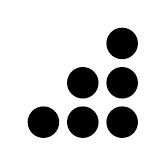
\begin{tikzpicture}
\foreach \x in {1,2,3}
	\foreach \y in {1,...,\x}
		\fill (.5*\x,.5*\y) circle (.2cm);
\end{tikzpicture}
&
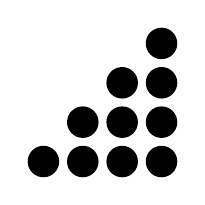
\begin{tikzpicture}
\foreach \x in {1,2,3,4}
	\foreach \y in {1,...,\x}
		\fill (.5*\x,.5*\y) circle (.2cm);
\end{tikzpicture}
\end{tabular}
\end{center}

Por la forma en que está definida esta sucesión de figuras, podemos constatar que el número de círculos negros en la $n$-ésima figura es exactamente igual a $s_n$.

Si deseamos obtener una fórmula cerrada para $s_n$ vamos a necesitar una herramienta más poderosa: el {\bf Principio de Inducción Matemática}, que veremos en la sección siguiente, aunque las figuras más arriba ya sugieren una fórmula.

\subsection{Progresiones: primer enfoque}

Entre las secuencias definidas por recurrencia, se distinguen dos que son particularmente importantes para las aplicaciones: las progresiones aritméticas y las progresiones geométricas.

\begin{itemize}
\item {\bf Progresión aritmética.} Dados dos números reales fijos: $a_0$, $d\in\R$, se define la siguiente sucesión:
\begin{eqnarray*}
a_0&=&a_0,\\
a_{n+1}&=&a_n+d,\textrm{ para }n\ge0.
\end{eqnarray*}
Vemos que cada término se separa del anterior por un valor constante: $d$, por lo tanto los primeros términos de la sucesión  son: $(a_0,a_0+d, a_0+2d,a_0+3d,\dots)$.\\
{\em Ejemplo: la sucesión de los números impares es una progresión aritmética:
\begin{eqnarray*}
i_0&=&1,\\
i_{n+1}&=&i_n+2,\textrm{ para }n\ge0.
\end{eqnarray*}
}
\item {\bf Progresión geométrica.} Dados dos números reales fijos: $g_0$, $r\in\R$, con $r\not\in\{0\}$, se define la siguiente sucesión:
\begin{eqnarray*}
g_0&=&g_0,\\
g_{n+1}&=&rg_n,\textrm{ para }n\ge0.
\end{eqnarray*}
Vemos que la razón entre dos términos sucesivos es igual a una constante: $r$, por lo tanto los primeros términos de la sucesión  son: $(g_0,rg_0, r^2g_0,r^3g_0,\dots)$.
{\em Ejemplo: la sucesión de las potencias de 10 es una progresión geométrica:
\begin{eqnarray*}
p_0&=&1,\\
p_{n+1}&=&10p_n,\textrm{ para }n\ge0.
\end{eqnarray*}
}
\end{itemize}

Indagaremos con más detalle en estas sucesiones en los siguientes capítulos.



\section{Inducción}


Si pones una hilera de dominós en forma vertical, lo suficientemente cerca los unos de los otros, la situación es inestable, si cae uno, todos los que siguen caerán, eso es claro ya que si uno cae, cae el que está al lado, pero entonces caerá el que está al lado de este, y así sucesivamente todos caerán. No necesitamos hacer el experimento, lo sabemos, una situación  que se enfrenta a iguales condiciones tiene iguales resultados es el caso de los dominós, sabemos lo que ocurrirá.
Pero mientras estén todos verticales, esa situación no tiene por qué cambiar, y seguirá así siempre.
Moraleja, para que caigan todos los dominós, se necesita que todos esté suficiente mente cerca de sus vecinos en la hilera y que caiga uno de los dominós de los extremos.

Esta es la metáfora del \emph{principio de inducción matemática}.
Para poder introducir esta herramienta, nos valdremos del concepto de ``\emph{función proposicional}'', visto en el capítulo anterior.


A veces nos encontramos con funciones proposicionales que siempre asignan un valor verdadero al argumento de entrada, estas corresponden a afirmaciones que son siempre ciertas, por ejemplo: \emph{$f(n):n+1\in\R$}, siempre que $n$ sea un número real, se cumple, por lo tanto siempre toma el valor de verdad {\tt V}.
En este caso podemos afirmar que $\forall n\in\R, f(n)$.
Este tipo de funciones proposicionales nos interesa pues describen las ``\emph{verdades}'' de nuestro sistema.

\medskip

\begin{ejercicio}\label{eje:ind}
Determine cuales de las siguientes funciones proposicionales son siempre verdaderas.
\begin{itemize}
\item $p:\R\rightarrow \{V,F\}$, definida por \emph{$p(x):-(-n)=n$}.
\item $p:\N\rightarrow \{V,F\}$, definida por \emph{$p(x):\left[(2^n\ge n^2)\vee(n\le 3)\right]$}.
\item $p:\R\rightarrow \{V,F\}$, definida por \emph{$p(x):2^{2n}-1$ es múltiplo de 3}.
\end{itemize}

Las funciones proposicionales que se cumplen siempre son \emph{propiedades} del sistema.

La primera la distinguimos pues es una de las propiedades del opuesto aditivo.
Las siguientes propiedades del ejemplo parecieran ser verdad, pero ¿cómo demostrarlas? 
\end{ejercicio}

Cuando se trata de una propiedad definida en los naturales, hay una herramienta que suele facilitar muchísimo el trabajo: el \emph{principio de inducción}.
Este consiste en demostrar primero que si la propiedad es verdadera para uno de los números, entonces también es verdadera para el siguiente número (equivale a demostrar que los dominoes están cerca unos de otros), y luego demostrar que la propiedad se cumple para el primer número (equivale a tumbar el primer dominó).
Con esto la implicancia demostrada se aplicará infinitas veces y habremos demostrado que la propiedad se cumple en todo $\N$.

\medskip

\begin{pp}
Dada una función proposicional $P:\N\rightarrow \{V,F\}$, si esta cumple que:
\begin{itemize}
\item $P(1)$ es verdadera, y
\item para cada $k\in\N$, si $P(k)$ es verdadera, entonces $P(k+1)$ también es verdadera,
\end{itemize}
entonces se tiene que $\forall n\in\N,\ P(n)$ es verdadera.
\end{pp}

\medskip

\begin{ejemplo}
En cierto modo, lo que hace el principio de inducción es cambiar la propiedad que queremos demostrar por otra que puede ser más simple. 
En el ejemplo anterior, la última propiedad es:
$$\forall n\in\N,\ 2^{2n}-1 \textrm{ es múltiplo de }3,$$
si usamos el principio de inducción lo que tenemos que demostrar es lo siguiente:
$$2^{2}-1\textrm{ es múltiplo de }3\quad\wedge\quad \forall n\in\N,\ \left[2^{2n}-1 \textrm{ es múltiplo de }3\Rightarrow 2^{2(n+1)}-1 \textrm{ es múltiplo de }3\right]$$
Esta nueva propiedad consiste en demostrar una implicancia, lo cual suele ser más fácil pues nos aporta una \emph{hipótesis}, que podemos usar.

Veámoslo en este mismo ejemplo.
Si intentamos demostrar directamente la propiedad,\break $\forall n\in\N,\ 2^{2n}-1 \textrm{ es múltiplo de }3,$ nos vemos sin ideas: por ejemplo $2^{2\cdot2}-1=16-1=15$, se cumple para n=2; $2^{2\cdot 4}-1=2^8-1=256-1=255=3\cdot85$, se cumple para $n=4$, pero ¿por qué? ¿qué pasa para $2^{40}-1$?

Pero si trabajamos la propiedad que nos da el principio de inducción tenemos que la primera parte es directa, ya que $2^{2}-1=4-1=3\textrm{ es múltiplo de }3$.
Intentemos ahora demostrar la segunda parte: 
$$\forall n\in\N,\ \left[2^{2n}-1 \textrm{ es múltiplo de }3\Rightarrow 2^{2(n+1)}-1 \textrm{ es múltiplo de }3\right]$$

Tomamos $n\in\N$ cualquiera, debemos demostrar la implicancia 
$$2^{2n}-1 \textrm{ es múltiplo de }3\Rightarrow 2^{2(n+1)}-1 \textrm{ es múltiplo de }3,$$
para lo cual suponemos que la hipótesis es cierta:
$$n\textrm{ es tal que cumple } 2^{2n}-1 \textrm{ es múltiplo de }3,$$
esto nos da algo de qué agarrarnos, nos dice que existe $k\in\N$ tal que $2^{2n}-1=3k$.
Ahora debemos demostrar la tesis: 
$$\textrm{debemos demostrar que }2^{2(n+1)}-1 \textrm{ es múltiplo de }3.$$
Pero para hacernos de ella contamos con la hipótesis, no estamos partiendo de nada.
Analizamos:
\begin{eqnarray*}
2^{2(n+1)}-1&=&2^{2n+2}-1\\
&=&2^22^{2n}-1\\
&=&4\cdot2^{2n}-1\\
&=&3\cdot2^{2n}+2^{2n}-1\\
&=&3\cdot2^{2n}+3k\\
&=&3(2^{2n}+k)
\end{eqnarray*}
el cual es un múltiplo de 3, con lo cual hemos demostrado la tesis, por lo tanto hemos demostrado la implicancia, y gracias al principio de inducción, hemos demostrado la propiedad: $$\forall n\in\N,\ 2^{2n}-1 \textrm{ es múltiplo de }3.$$
\end{ejemplo}

\begin{ejercicio}
Intente demostrar la segunda propiedad del ejercicio~\ref{eje:ind} usando el principio de inducción. Para ello se recomienda tomar como caso inicial $n=4$.
\end{ejercicio}

No siempre el principio de inducción es necesario, no siempre ayuda, pero hay una clase de problemas para los cuales no hay otra opción: demostrar propiedades de objetos definidos por \emph{recurrencia}.

Como los términos de una recurrencia no están dados por una fórmula cerrada, si no que están en función de los términos anteriores, no es posible demostrar nada de manera directa respecto a estas. Pero el principio de inducción se adapta de maravilla para trabajar con estas secuencias.

\medskip

\begin{ejemplo}\label{eje:sn}
Considere $(s_n)_{n\in\N}$ definida como sigue:

\begin{eqnarray*}
s_1&=&1,\\
s_n&=&s_{n-1}+n,\textrm{ para }n\ge2,
\end{eqnarray*}

entonces se cumple para todo $n\in\N$ que:
$$P(n): s_n=\frac{n(n+1)}{2}.$$

Verificamos que para el primer término es verdad.
\begin{eqnarray*}
\frac{1\cdot2}{2}&=&\frac{2}{2}=1=s_1.
\end{eqnarray*}
Demostremos ahora el \emph{paso de inducción}: tomamos un $n\ge3$ cualquiera y asumimos que se cumple $P(n)$, es decir que: $s_n=\frac{n(n+1)}{2}$.
Entonces trabajamos $P(n+1)$ : $s_{n+1}=\frac{(n+1)(n+2)}{2}$.
\begin{eqnarray*}
s_{n+1}&=&s_n+(n+1) \qquad\textrm{aplicando la definición de la recurrencia}\\
&=&\frac{n(n+1)}{2}+n+1 \qquad\textrm{aplicando la hipótesis de inducción}\\
&=&\frac{n(n+1)+2n+2}{2}\\
&=&\frac{n(n+1)+2(n+1)}{2}\\
&=&\frac{(n+1)(n+2)}{2}
\end{eqnarray*}
Por lo tanto, por el principio de inducción hemos demostrado que 
$$\forall n\in\N,\ P(n):s_n=\frac{n(n+1)}{2}.$$
\end{ejemplo}

El principio de inducción supone una aplicación del paso de inducción tantas veces como sea necesario hasta llegar al término $n$-ésimo, esa aplicación no la hace quien usa el principio de inducción, si no que se asume hecho ya que al demostrar el paso de inducción se ha demostrado que se puede hacer, y con eso basta.

Sabemos que la propiedad es verdadera para $n=10$ ya que sabemos que es cierta para el primer término y que luego podemos aplicar el paso de inducción para $n=1$, demostrando con eso que es cierta para el segundo término, y podemos aplicar el paso de inducción para $n=2$ lo cual nos dice que es cierta para el tercer término, etc.. No necesitamos hacer todos esos pasos pues ya entendimos la técnica, sabemos que se pueden hacer y eso nos asegura la propiedad para $n=10$ y para cualquier número natural.

Mediante el principio de inducción es posible demostrar las propiedades de sumatorias.

\medskip

\begin{prop} Dadas dos secuencias $(a_j)_{j\in\N}$ y $(b_j)_{j\in\N}$, dado $\lambda\in\R$ y dados $1\le l\le m\le n$, se cumplen las siguientes propiedades.
\begin{enumerate}
\item\label{it:0} ${\displaystyle \sum_{j=m}^n 0=0}$
\item\label{it:cte} ${\displaystyle  \sum_{j=m}^n 1=n-m+1}$
\item\label{it:ponderacion} ${\displaystyle  \sum_{j=m}^n \lambda a_j=\lambda\left(\sum_{j=m}^n a_j\right)}$
\item\label{it:suma} ${\displaystyle  \sum_{j=m}^n (a_j+b_j)=\left(\sum_{j=m}^n a_j\right)+\left(\sum_{j=m}^n b_j\right)}$
\item\label{it:separacion} ${\displaystyle  \sum_{j=l}^n a_j=\left(\sum_{j=l}^m a_j\right)+\left(\sum_{j=m+1}^n a_j\right)}$
\item\label{it:variable} Para cualquier $i\in\N$, ${\displaystyle  \sum_{j=m}^n a_j=\sum_{j=m-i}^{n-i} a_{j+i}}$
\item\label{it:telescopica} ${\displaystyle \sum_{j=m}^n (a_{j+1}-a_j)=a_{n+1}-a_m}$
\end{enumerate}
\end{prop}
{\bf Demostración.}
La mayoría de estas propiedades son intuitivas si uno tiene en cuenta que la sumatoria es simplemente una suma de muchos términos, por lo tanto estas propiedades podrían verse como una simple extensión de propiedades de la suma, aunque en rigor, dado que la suma se define por recurrencia, éstas deben ser demostradas por inducción.\\

Demostremos la propiedad 7 como ejemplo. Lo haremos por inducción.\\
(Base de inducción) $n=m$: ${\displaystyle \sum_{j=m}^m (a_{j+1}-a_j)=a_{m+1}-a_m=a_{n+1}-a_m}$, lo cual es verdad directamente de hecho que $n=m$.\\
(Paso de inducción) Si ${\displaystyle \sum_{j=m}^n (a_{j+1}-a_j)=a_{n+1}-a_m}$, entonces ${\displaystyle \sum_{j=m}^{n+1} (a_{j+1}-a_j)=a_{n+2}-a_m}$.\\
Asumimos la hipótesis: ${\displaystyle \sum_{j=m}^n (a_{j+1}-a_j)=a_{n+1}-a_m}$\\
Buscamos demostrar la tesis: ${\displaystyle \sum_{j=m}^{n+1} (a_{j+1}-a_j)=a_{n+2}-a_m}$.\\
\begin{eqnarray*}
  \sum_{j=m}^{n+1} (a_{j+1}-a_j)&=& \left(\sum_{j=m}^{n} (a_{j+1}-a_j)\right) +(a_{n+2}-a_{n+1})\qquad \textrm{de la definición de sumatoria}\\
  &=& \left(a_{n+1}-a_m\right) +a_{n+2}-a_{n+1}\qquad \textrm{de la hipótesis}\\
  &=&a_{n+2} -a_m\\
\end{eqnarray*}
Que era lo que queríamos demostrar.
\hfill $\Box$

\subsection{Progresiones: segunda parte}


Cuando definimos las progresiones, establecimos que se pueden definir tanto por recurrencia como mediante una fórmula cerrada. Lo cual es muy útil pues en general la definición por recurrencia habla del proceso por el cual se genera la sucesión de números, mientras que la fórmula cerrada nos permite calcularla, predecirla.
La fórmula cerrada de las progresiones, en realidad se demuestra formalmente por inducción, y lo haremos a continuación

\medskip

\begin{prop}
Dados $a_0, d\in\R$ fijos, el término general de la progresión aritmética definida como sigue:
\begin{eqnarray*}
a_0&=&a_0,\\
a_{n+1}&=&a_n+d,\textrm{ para }n\ge0.
\end{eqnarray*}
se obtiene con la fórmula $a_n=a_0+nd$.
\end{prop}
{\bf Demostración.}
Vamos a demostrar por inducción que la fórmula se cumple.
(Base de inducción) $n=0$: $a_0=a_0+0=a_0+0d=a_0+nd$, dado que $n=0$.\\
(Paso de inducción) Si $a_n=a_0+nd$, entonces $a_{n+1}=a_0+(n+1)d$\\
Asumimos la hipótesis: $a_n=a_0+nd$\\
Buscamos demostrar la tesis: $a_{n+1}=a_0+(n+1)d$\\
\begin{eqnarray*}
  a_{n+1}&=&a_n+d \qquad \qquad \textrm{de la definición de la progresión aritmética}\\
  &=& a_0+nd+d  \qquad \textrm{de la hipótesis de inducción}\\
  &=& a_0+(n+1)d \qquad \textrm{sacando a $d$ como factor común }
\end{eqnarray*}
\hfill $\Box$


\begin{prop}
Dados $g_0, r\in\R\setminus\{0\}$ fijos, el término general de la progresión geométrica definida como sigue:
\begin{eqnarray*}
g_0&=&g_0,\\
g_{n+1}&=&rg_n,\textrm{ para }n\ge0.
\end{eqnarray*}
se obtiene con la fórmula $g_n=g_0r^n$.
\end{prop}
{\bf Demostración.}
Vamos a demostrar por inducción que la fórmula se cumple.
(Base de inducción) $n=0$: $g_0=g_01=g_0r^0=g_0r^n$, dado que $n=0$.\\
(Paso de inducción) Si $g_n=g_0r^n$, entonces $g_{n+1}=g_0r^{n+1}$\\
Asumimos la hipótesis: $g_n=g_0r^n$\\
Buscamos demostrar la tesis: $g_{n+1}=g_0r^{n+1}$\\
\begin{eqnarray*}
  g_{n+1}&=&rg_n \qquad \qquad \textrm{de la definición de la progresión geométrica}\\
  &=& r g_0r^n  \qquad \textrm{de la hipótesis de inducción}\\
  &=& g_0r^{n+1} \qquad \textrm{de la propiedad de la multiplicación de potencias}
\end{eqnarray*}
\hfill $\Box$

La progresiones tienen múltiples aplicaciones en el mundo financiero, allí puede ser interesante sumar los términos de una progresión, por ejemplo cuando estos representan un dinero ahorrado cada año, o una ganancia mensual.

\begin{prop}
Dados $a_0, d\in\R$ fijos, si consideramos la progresión aritmética definida como sigue:
\begin{eqnarray*}
a_0&=&a_0,\\
a_{n+1}&=&a_n+d,\textrm{ para }n\ge0.
\end{eqnarray*}
entonces se cumple
$$\sum_{n=0}^Na_n=\sum_{n=0}^N(a_0+nd)=(N+1)a_0+d\frac{N(N+1)}{2}.$$
\end{prop}
{\bf Demostración.}
Podemos hacerla usando las propiedades de las sumatorias y lo calculado en el ejercicio~\ref{eje:sn}.
\begin{eqnarray*}
\sum_{n=0}^Na_n&=&\sum_{n=0}^N(a_0+nd)\qquad \textrm{de la propiedad~\ref{it:suma} de sumatorias}\\
&=&\sum_{n=0}^Na_0+\sum_{n=0}^N nd\qquad \textrm{de la propiedad~\ref{it:cte} y~\ref{it:ponderacion} de sumatorias}\\
&=&(N+1)a_0+d\sum_{n=0}^N n\qquad \textrm{de la propiedad~\ref{it:separacion}}\\
&=&(N+1)a_0+d\left(\sum_{n=1}^N n+0\right)\qquad \textrm{ya que 0 es neutro aditivo}\\
&=&(N+1)a_0+d\sum_{n=1}^N n\qquad \textrm{del ejercicio~\ref{eje:sn}}\\
&=&(N+1)a_0+d\frac{N(N+1)}{2}
\end{eqnarray*}
\hfill $\Box$

\begin{prop}
Dados $g_0, r\in\R\setminus\{0\}$ fijos, si consideramos la  progresión geométrica definida como sigue:
\begin{eqnarray*}
g_0&=&g_0,\\
g_{n+1}&=&rg_n,\textrm{ para }n\ge0.
\end{eqnarray*}
entonces se cumple
$$\sum_{n=0}^Ng_n=\sum_{n=0}^Ng_0r^n=g_0\frac{1-r^{N+1}}{1-r}$$
\end{prop}
{\bf Demostración.}
Para calcular esta suma, haremos uso de un truco que es muy útil a la hora de calcular sumas de este tipo, y vale la pena recordar, pues además permitirá recordar la fórmula si es que se les llega a olvidar.
Lo primero es observar que por la propiedad de~\ref{it:ponderacion} se cumple:
$$\sum_{n=0}^Ng_n=\sum_{n=0}^Ng_0r^n=g_0\sum_{n=0}^Nr^n.$$
Por lo tanto, sólo nos interesa calcular lo que denominaremos ${\displaystyle S_N=\sum_{n=0}^Nr^n}$.\\
Primero observamos lo siguiente, gracias a la definición de sumatoria.
$$S_{N+1}=\sum_{n=0}^{N+1}r^n=\sum_{n=0}^Nr^n+r^{N+1}=S_N+r^{N+1}$$
Pro dado que estamos sumando potencias, podemos también observar lo siguiente, gracias a las propiedades de~\ref{it:separacion},~\ref{it:variable} y~\ref{it:ponderacion}.
$$S_{N+1}=\sum_{n=0}^{N+1}r^n=1+\sum_{n=1}^{N+1}r^n=1+\sum_{n=0}^{N}r^{n+1}=1+r\sum_{n=0}^{N}r^{n}=1+rS_N$$
Igualando las dos expresiones obtenidas para $S_{N+1}$ obtenemos:
$$S_N+r^{N+1}=1+rS_N.$$
De donde es posible despejar $S_N$.
\begin{eqnarray*}
S_N+r^{N+1}&=&1+rS_N\qquad /-r^{N+1}-rS_N\\
S_N-rS_N&=&1-r^{N+1}\qquad \textrm{factorizando}\\
S_N(1-r)&=&1-r^{N+1}\qquad /\times\frac{1}{1-r}\\
S_N&=&\frac{1-r^{N+1}}{1-r}
\end{eqnarray*}
Por lo tanto
$$\sum_{n=0}^Ng_n=g_0\sum_{n=0}^Nr^n=g_0S_N=g_0\frac{1-r^{N+1}}{1-r},$$
que era lo que se quería demostrar.
\hfill $\Box$

La inducción es práctica para demostrar muchas cosas, algunas muy bonitas, en este nivel, sólo haremos demostraciones simples con números, pero a quienes esta materia les parezca atractiva, hay muchísimas aplicaciones lúdicas del principio de inducción, así como también muchas aplicaciones a las ciencias de la computación.



\subsection{Inducción fuerte}

Cuando partimos de la base de inducción e hipotéticamente hemos aplicado el paso de inducción $n$ veces, ya hemos demostrado la propiedad para todos los términos anteriores a $n$.
Esto nos da otra forma del principio de inducción que es más poderosa y avanzada.

\medskip

\begin{pp}[{\bf fuerte}]
Dada una función proposicional $P:\N\rightarrow \{V,F\}$, si esta cumple que:
\begin{itemize}
\item $P(1)$ es verdadera, y
\item para cada $k\in\N$, si $P(j)$ es verdadera para todo $j\in\{1,\dots,k\}$, entonces $P(k+1)$ también es verdadera,
\end{itemize}
entonces se tiene que $\forall n\in\N,\ P(n)$ es verdadera.
\end{pp}

En esta versión el paso de inducción tiene una hipótesis más fuerte, podemos usar la propiedad para todos los valores anteriores al que estamos estudiando. 
Ilustremos esto con la serie de Fibonacci.

\begin{ejemplo}
Considerando la serie de Fibonacci antes definida, $(f_n)_{n\in\N}$ se cumple lo siguiente para todo $n\in\N$:
$$ f_n\textrm{ es par  si y solo si $n$ es múltiplo de 3}$$

Miremos primero un poco la serie de Fibonacci para hacernos de la idea detrás de la demostración que vamos a hacer.

\begin{center}
\begin{tabular}{c|cccccccc}
$n$&1&2&\circled{3}&4&5&\circled{6}&7&8\\\hline
$f_n$&1&1&\circled{2}&3&5&\circled{8}&13&21
\end{tabular}
\end{center}

Vemos que la propiedad se cumple par los primeros 8 términos, y podemos enarbolar una razón: cuando los dos términos consecutivos son impares, el término que viene debe ser par; por su parte, el término subsiguiente será suma de un par más un impar, por lo tanto será impar; y lo mismo pasará con el que sigue, etc..
Estamos listas y listos para la demostración, tenemos la idea.

Tomemos $n\ge 3$ arbitrario, y supongamos ahora que se cumple que $ f_j$  es par  si y solo si $j$ es múltiplo de 3 para todo $j\le n$, y estudiemos la paridad de $f_{n+1}$ (hipótesis). 

Observamos que respecto a la divisibilidad por 3, existen solo 3 tipos de números: los múltiplos de 3, los que son múltiplo de 3 más 1 y los que son múltiplo de 3 más 2. Por lo tanto tres casos aparecen:
\begin{itemize}
\item $n+1$ es múltiplo de 3: en este caso es claro que ni $n$ ni $n-1$ son múltiplos de 3, por lo tanto, la hipótesis nos dice que $f_n$ y $f_{n-1}$ son impares, por lo tanto $f_{n+1}=f_n+f_{n-1}$ es par.
\item $n+1$ no es múltiplo de 3, pero $n$ sí lo es: en este caso es claro que $n-1$ no es múltiplo de 3, por lo tanto, la hipótesis nos dice que $f_n$ es par pero $f_{n-1}$ es impar, por lo tanto $f_{n+1}=f_n+f_{n-1}$ es impar.
\item $n+1$ no es múltiplo de 3, pero $n-1$ sí lo es: en este caso es claro que  $n$ no es múltiplo de 3, por lo tanto, la hipótesis nos dice que $f_n$ es impar y $f_{n-1}$ es par, por lo tanto $f_{n+1}=f_n+f_{n-1}$ es impar.
\end{itemize}
Hemos demostrado que $ f_{n+1}$es par  si y solo si $n+1$ es múltiplo de 3 a partir de suponer que $f_j$ es par  si y solo si $j$ es múltiplo de 3, para todo $j\le n$.

Por el principio de inducción fuerte hemos demostrado que para todo $n\in\N$, $f_n$ es par  si y solo si $n$ es múltiplo de 3.
\end{ejemplo}


\section{Coeficientes combinatoriales}


Supongamos que se tiene el conjunto $A = \{1,2,3,4,5\}$. 
Se quiere contar cu\'antos subconjuntos de cardinalidad 2 tiene $A$.
Para ello puede tenerse en cuenta que existen 5 formas distintas de escoger el primer elemento de un posible subconjunto y, una vez escogido \'el, s\'olo existen 4 formas distintas de escoger el segundo. 
Pero adem\'as debemos considerar que los conjuntos $\{1,2\}$ y $\{2,1\}$ son iguales.
Por tanto, existen $\dfrac{5\cdot 4}{2}$ subconjuntos de $A$ de cardinalidad 2.
Ellos son
\[
	\{1,2\}, \{1,3\}, \{1,4\}, \{1,5\}, \{2,3\}, \{2,4\}, \{2,5\},
	\{3,4\}, \{3,5\}, \{4,5\}.
\]

El mismo razonamiento puede aplicarse a subconjuntos de tamaño $k$ dentro de un conjunto de tamaño $n$: el primer elemento puede elegirse de $n$ formas distintas, el segundo de $n-1$ maneras distintas, el tercero de $n-2$, etc.. hasta de $n-k+1$ maneras se puede elegir el último de los $k$ elementos que se agregue al conjunto, total:

$$ n\cdot (n-1) \cdot (n-2) \cdots (n-k+1) $$

Igual que en el caso de 2 elementos, acá estamos repitiendo conjuntos que son iguales solo que sus elementos fueron escogidos en otro orden.
Por esta razón, debemos dividir por el número de ordenamientos distintos que hay de $k$ elementos.
El cual es posible demostrar que es $k!$, así el número total de conjuntos de $k$ elementos en un conjunto de $n$ elementos es:


\[
	\binom{n}{k} = \frac{n(n-1)(n-2)...(n-k+1)}{k!}  = \frac{n!}{(n-k)!k!}
\]

Este n\'umero recibe el nombre de {\em coeficiente binomial}.

\medskip

\begin{prop}
\begin{enumerate}
\item $\binom{n}{0} = \binom{n}{n} = 1$ 
\item $\binom{n}{1} = n$ 
\item $\binom{n}{k} = \binom{n}{n-k}$
\item $\binom{n+1}{k+1} = \binom{n}{k} + \binom{n}{k+1}$
\end{enumerate}
\end{prop}
{\bf Demostración.}
\begin{enumerate}
\item ${n\choose 0}=\frac{n!}{n!0!}=1$ y ${n\choose n}=\frac{n!}{0!n!}=1$
\item ${n\choose 1}=\frac{n!}{(n-1)!1!}=n$
\item ${n\choose k}=\frac{n!}{k!(n-k)!}=\frac{n!}{(n-k)!k!}={n\choose n-k}$
\item
  \begin{align*}
    \binom{n}{k} + \binom{n}{k+1} &= \frac{n!}{(n-k)!k!} + \frac{n!}{(n-k-1)!(k+1)!},\\
    &= \frac{n!(k+1) + n!(n-k)}{(k+1)!(n-k)!},\\
    &= \frac{n!(k+1+n-k)}{(k+1)!(n-k)!},\\
    &= \frac{(n+1)!}{(k+1)!(n-k)!},\\
    &= \frac{(n+1)!}{(k+1)!(n+1-(k+1))!},\\
    &= \binom{n+1}{k+1}.
  \end{align*}
\end{enumerate}
\hfill $\Box$

Podemos interpretar cada una de estas propiedades en términos de lo que representan como sigue.
\begin{enumerate}
\item Esta propiedad nos dice que el \'unico subconjunto de un conjunto $A$ de cardinalidad $n$ que tiene cardinalidad 0 es el conjunto vac\'{\i}o y el \'unico que tiene cardinalidad $n$ es el propio $A$.
\item La segunda propiedad se entiende ya que hay $n$ subconjuntos de cardinalidad 1.
\item Esta propiedad se explica ya que cuando se escogen $k$ elementos de un conjunto, los que quedan sin escoger conforman otro conjunto $n-k$ elementos, por lo tanto se contabilizan la misma manera.
\item La última propiedad es la más complicada de interpretar, pero intentémoslo.
  Lo primero es tomar un conjunto $A$ con $n+1$ elementos, queremos contar cuántos subconjuntos hay de $k+1$ elementos dentre de este conjunto.
  Pero deseamos hacerlo basándonos en los coeficientes combinatoriales que tenemos para conjuntos de $n$ elementos.
  Entonces escogemos un elementos cualquiera de $A$ y lo sacamos.
  Con los elementos restantes puedo hacer un conjunto de $k+1$ elementos que es lo que queremos contabilizar, esto nos da ${n\choose k+1}$ conjuntos diferentes.
  Pero también podríamos escoger un conjunto con solo $k$ elementos y a este agregarle el elemento de $A$ que habíamos apartado, así obtendremos conjuntos con $k+1$ elementos que serán distintos de los que escogimos antes, en total, habrán ${n\choose k}$ de estos conjuntos.
  No hay más posibilidades, así que el número total de conjuntos de $k+1$ elementos de $A$: ${n+1\choose k+1}$ es la suma de estos dos números: ${n\choose k+1}+{n\choose k}$.
\end{enumerate}
    
El ítem 4 nos da una forma recursiva de calcular $\binom{n}{k}$ para cualquier
par de $n,k \in \N \cup \{0\}, n \ge k$. Por ejemplo,
\begin{eqnarray*}
  \binom{5}{3} &=& \binom{4}{3} + \binom {4}{2},\\
  &=& 4 + \binom{3}{2} + \binom{3}{1},\\
  &=& 4 + 3 + 3,\\
  &=& 10
\end{eqnarray*}
En esto se basa el tri\'angulo de Pascal,

\begin{center}
\begin{tabular}{ccccccccccc}\\
	& & & & & $\binom{0}{0}$ & & & & &\\
	& & & & $\binom{1}{0}$ & & $\binom{1}{1}$ & & & &\\
	& & & $\binom{2}{0}$ & & $\binom{2}{1}$ & & $\binom{2}{2}$ & & &\\
	& & $\binom{3}{0}$ & & $\binom{3}{1}$ & & $\binom{3}{2}$ & & $\binom{3}{3}$ & &\\
	& $\binom{4}{0}$ & & $\binom{4}{1}$ & & $\binom{4}{2}$ & & $\binom{4}{3}$ & & $\binom{4}{4}$ &\\
	$\binom{5}{0}$ & & $\binom{5}{1}$ & & $\binom{5}{2}$ & & $\binom{5}{3}$ & & $\binom{5}{4}$ & & $\binom{5}{5}$
\end{tabular}
\end{center}

\medskip
lo cual se convierte en
\begin{center}
\begin{tabular}{ccccccccccc}\\
	& & & & & $1$ & & & & &\\
	& & & & $1$ & & $1$ & & & &\\
	& & & $1$ & & $2$ & & $1$ & & &\\
	& & $1$ & & $3$ & & $3$ & & $1$ & &\\
	& $1$ & & $4$ & & $6$ & & $4$ & & $1$ &\\
	$1$ & & $5$ & & $10$ & & $10$ & & $5$ & & $1$
\end{tabular}
\end{center}

\medskip

\subsection{Teorema del binomio}

Los coeficientes binomiales son \'utiles al calcular un binomio elevado a una
potencia natural.

Para verlo más claro, vamos a redefinir la potencia de un número por recurrencia, esto reafirmará la noción que ya conocemos y nos permitirá trabajar con ella a trevés del principio de inducción.

\begin{eqnarray*}
  x^0 &=& 1,\\
  x^n &=& x^{n-1}x, \textrm{ si }n\ge1
\end{eqnarray*}

Si queremos calcular la potencia de un ``binomio'' se complican las cosas, pues la combinatoria ``explota'', veamos.

\begin{eqnarray*}
  (x+y)^0 &=& 1\\
  (x+y)^1 &=& x+y\\
  (x+y)^2 &=& (x+y)(x+y)\\
  &=& xx + xy + yx + yy\\
  &=& x^2+2xy+y^2\\
  (x+y)^3 &=& (x+y)(x+y)(x+y)\\
  &=& xxx+xxy+xyx+xyy+yxx+yxy+yyx+yyy\\
  &=& x^3+3x^2y+3xy^2+y^3
\end{eqnarray*}

Observe que al multiplicar los binomios el resultado es la suma de todos los productos posibles.
Por ejemplo el producto entre tres binomios el resultado es la suma de todos los productos posibles de tres n\'umeros con el primero en el primer binomio, el
segundo en el segundo binomio y el tercero, en el tercer binomio.

Observamos que en todos los términos la suma de las potencias de $x$ y de $y$ es la misma: 3 en el caso del cubo, 2 en el caso del cuadrado.
Esto es lógico ya que siempre estaremos multiplicando 3 cosas en el caso del cubo, pues de todas formas es el producto de 3 binomios.

Una vez que desplegamos todas las combinaciones posibles, nos damos cuenta que algunos términos son semejantes, gracias a la conmutatividad del producto en los reales, y por lo tanto los podemos sumar, y allí aprece un número que los pondera, y que caracteriza al producto notable en cuestión. ¿Pero cómo calcular ese número?

Esta pregunta  nos lleva de regreso al coeficiente combinatorial, ya que si nos preguntamos cuántas combinaciones darán lugar a productos semejantes, por ejemplo, cuántas veces aparecerá el término $x^2y$ en el cubo del binomio, la pregunta se traduce en decidir de cuántas maneras puedo escoger 2 veces la variable x dentro de los 3 binomios que estamos multiplicando, por ejemplo puedo escogerla una vez del primer binomio y una vez del segunda, obtengo el término $xxy$, pero también puedo escogerla una vez del primero y otra del tercero, obtengo el producto $xyx$, etc..

Entonces la pregunta de cuántas veces aparecerá un término semejante a $x^y$ en el cubo del binomio $(x+y)^3$ equivale a la pregunta de cuántos subconjuntos de tamaño 2 hay en un conjunto de 3 elementos, la respuesta es ${3\choose2}=3$.

Veámoslo más generalmente.
El producto
\[
	(x+y)^n = (x+y)(x+y)\cdots(x+y)
\]
es la suma de todos los productos entre $n$ n\'umeros, con el primero en el primer binomio, el segundo en el segundo binomio, el tercero, en el tercer binomio y as\'{\i} sucesivamente.
Ac\'a los binomios son iguales, por tanto,
$(x+y)^n$ es la suma de todos los productos de la forma 
\[
	x^ky^{n-k},\quad k \in \{0,1,\ldots,\,n\}
\]
donde $x$ es escogida de algunos binomios e $y$ de los restantes. 
Hay $\binom{n}{0}$ formas de escoger solo a $x$ en todos los binomios, por tanto, hay $\binom{n}{0}$ productos de la forma $x^ny^0$.
Hay $\binom{n}{1}$ formas de escoger a $y$ de solo uno de los $n$ binomios, por tanto, hay $\binom{n}{1}$ productos de la forma $X^{n-1}y^{1}$.
En general, hay $\binom{n}{k}$ formas de escoger $x$ exactamente $k$ veces en el conjunto de los $n$ binomios, por lo tanto, hay $\binom{n}{k}$ productos de la forma $x^ky^{n-k}$.
Sumando todos ellos se obtiene la f\'ormula de un binomio elevado a $n \in \N$.

\begin{thm}[Binomio de Newton]
  Dados dos números reales cualesquiera $x$, $y\in\R$ y un natural $n$, se cumple lo siguiente.
	$$(x+y)^n = \sum_{k=0}^n \binom{n}{k}x^{n-k}y^{k}$$
\end{thm}
{\bf Demostración.}
Lo demostraremos usando el principio de inducción.
\begin{itemize}
\item (Base de inducción) $n=1$:
  $$(x+y)^1=x+y=\sum_{k=0}^1{1\choose k}x^{1-k}y^{k}=\underbrace{{1\choose0}x^1y^0}_{k=0}+\underbrace{{1\choose1}x^0y^1}_{k=1}=1x+1y=x+y$$
\item (Paso de inducción) Suponemos que se cumple para un $n$ dado (hipótesis) y lo demostramos para $n+1$\footnote{Esta demostración usa varios trucos y aplica casi todas las propiedades de las sumatorias, leerla con atención es una buena práctica para aprender a manejar sumatorias.}.
\begin{align*}
  (x+y)^{n+1} &= (x+y)^n (x+y)\\
  &= \left(\sum_{k=0}^n \binom{n}{k}x^{n-k}y^{k}\right) (x+y)\\
  &= \left(\sum_{k=0}^n \binom{n}{k}x^{n-k}y^{k}(x+y)\right)\\
  &= \left(\sum_{k=0}^n \binom{n}{k}x^{n-k+1}y^{k}\right)+
  \left(\sum_{k=0}^n \binom{n}{k}x^{n-k}y^{k+1}\right)\\
  &= \left(\sum_{k=0}^n \binom{n}{k}x^{n-k+1}y^{k}\right)+
  \left(\sum_{k'=1}^{n+1} \binom{n}{k'-1}x^{n-(k'-1)}y^{k'}\right)\\
  &= {n\choose 0} x^{n+1}y^0+\left(\sum_{k=1}^n \binom{n}{k}x^{n-k+1}y^{k}\right)+
  \left(\sum_{k=1}^{n} \binom{n}{k-1}x^{n-(k-1)}y^{k}\right)+{n\choose n}x^{n-n}y^{n+1}\\
  &= x^{n+1}+\left(\sum_{k=1}^n \left[\binom{n}{k}+ \binom{n}{k-1}\right]x^{n-(k-1)}y^{k}\right)+y^{n+1}\\
\end{align*}

\begin{align*}
  \phantom{(x+y)^{n+1}}
  &= x^{n+1}+\left(\sum_{k=1}^n \binom{n+1}{k}x^{n+1-k}y^{k}\right)+y^{n+1}\phantom{  \left(\sum_{k=1}^{n} \binom{n}{k-1}x^{n-(k-1)}y^{k}\right)+{n\choose n}x^{n-n}y^{n+1}}\\
  &= \left(\sum_{k=0}^{n+1} \binom{n+1}{k}x^{n+1-k}y^{k}\right)\\
\end{align*}
Que era justo lo que queríamos demostrar. \hfill $\Box$
\end{itemize}

\medskip

\begin{ejemplo}
  Por ejemplo,
  \begin{align*}
    (x+y)^5 = \binom{5}{0}x^5 + \binom{5}{1}x^4y + \binom{5}{2}x^3y^2 + \binom{5}{3}x^2y^3 + \binom{5}{4} xy^4 + \binom{5}{5}y^5
  \end{align*}
  que, con ayuda del tri\'angulo de Pascal, obtenemos 
  \[
  x^5 + 5x^4y + 10x^3y^2 + 10x^2y^3 + 5xy^4 + y^5.
  \]
\end{ejemplo}

\begin{ejemplo}
  \begin{eqnarray*}
    (x+7)^4&=&\binom{4}{0}x^4 + \binom{4}{1}x^37^1 + \binom{4}{2}x^27^2 + \binom{4}{1}x^17^3 + \binom{4}{0}7^4\\
    &=& x^4+4x^37+6x^27^2+4x7^3+ 7^4\\
    &=& x^4+28x^3+294x^2+1372x+ 2401
  \end{eqnarray*}
\end{ejemplo}

